\section[LMs]{Lineare Modelle}

%\begin{frame}
%  {Übersicht}
%  \begin{itemize}[<+->]
%    \item weitere Korrelationen und Signifikanztests dafür
%    \item vom Messen der Korrelation zum Vorhersagemodell
%    \item lineare Modellanpassung mit mehreren Unabhängigen
%    \item ANOVA als Sonderfall des LM
%  \end{itemize}
%\end{frame}

\begin{frame}
  {Literatur}
  \begin{itemize}
    \item \cite{GravetterWallnau2007}
    \item \cite{ZuurEa2009}
    \item \cite{MaxwellDelaney2004}
  \end{itemize}
\end{frame}

\begin{frame}
  {Übersicht}
  \begin{itemize}[<+->]
    \item Pearson-Korrleation ($r$, $r^2$)
    \item Siginifikanztests mit Korrelationen
    \item Unterschied von Pearsons $r$ zu Spearmans Rang-Korrelation
    \item Unterschiede zwischen Korrelation und Regression
    \item Berechnung linearer Regressionsmodelle
    \item Signifikanztests für Modell und Koeffizienten
%    \item Vergleich linearer Modelle mit ANOVAs
  \end{itemize}
\end{frame}

\subsection{Korrelation und Signifikanz}

\begin{frame}
  {Korrelationen | Zusammenhänge zwischen numerischen Variablen}
  Bivariate Korrelationskoeffizienten | \orongsch{ab Ordinalskala}\\
  \begin{center}
    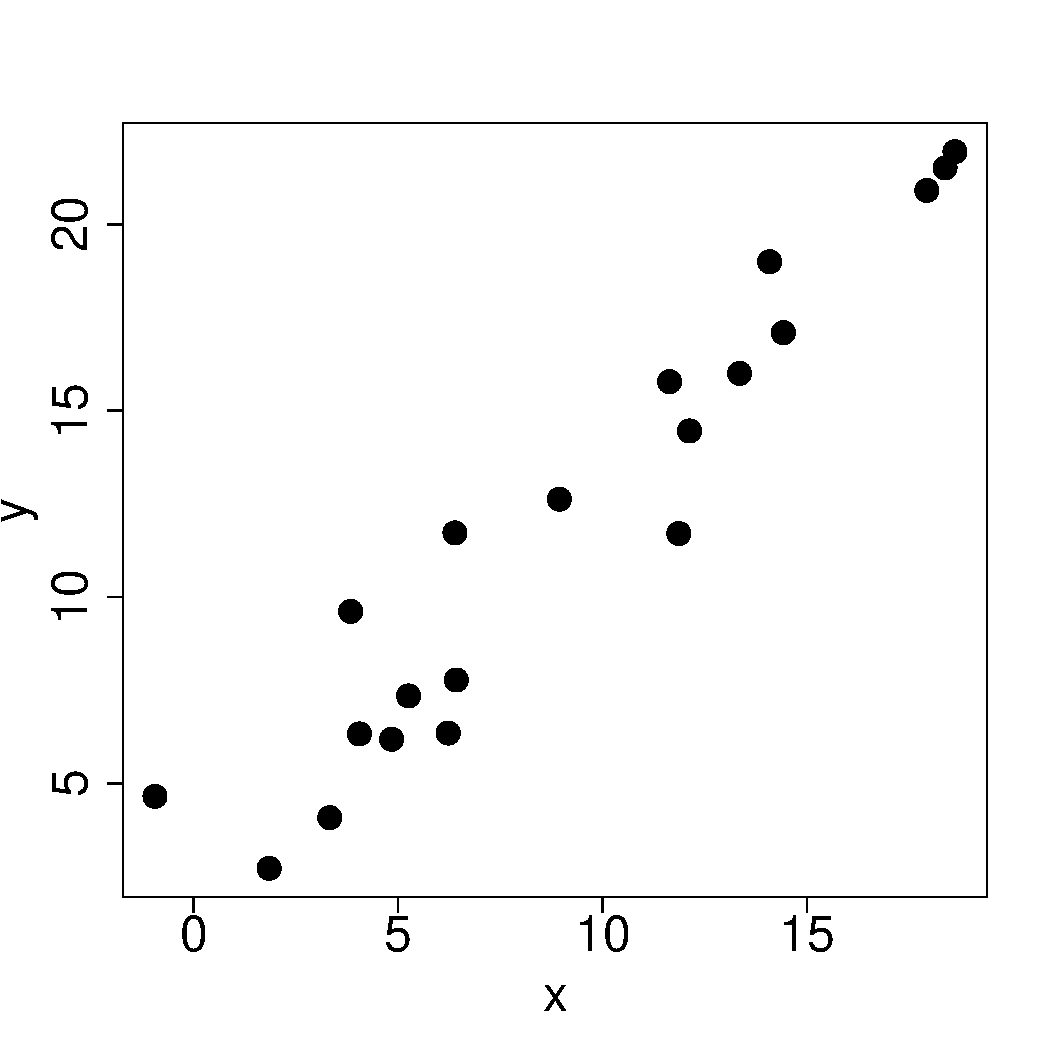
\includegraphics[height=0.7\textheight]{graphics/corrplot}
  \end{center}
\end{frame}


\begin{frame}
  {Kovarianz | Illustration 1}
  Koordinate von $\langle\bar{x},\bar{y}\rangle$ | Mittel der beiden gemessenen Variablen\\
  \begin{center}
    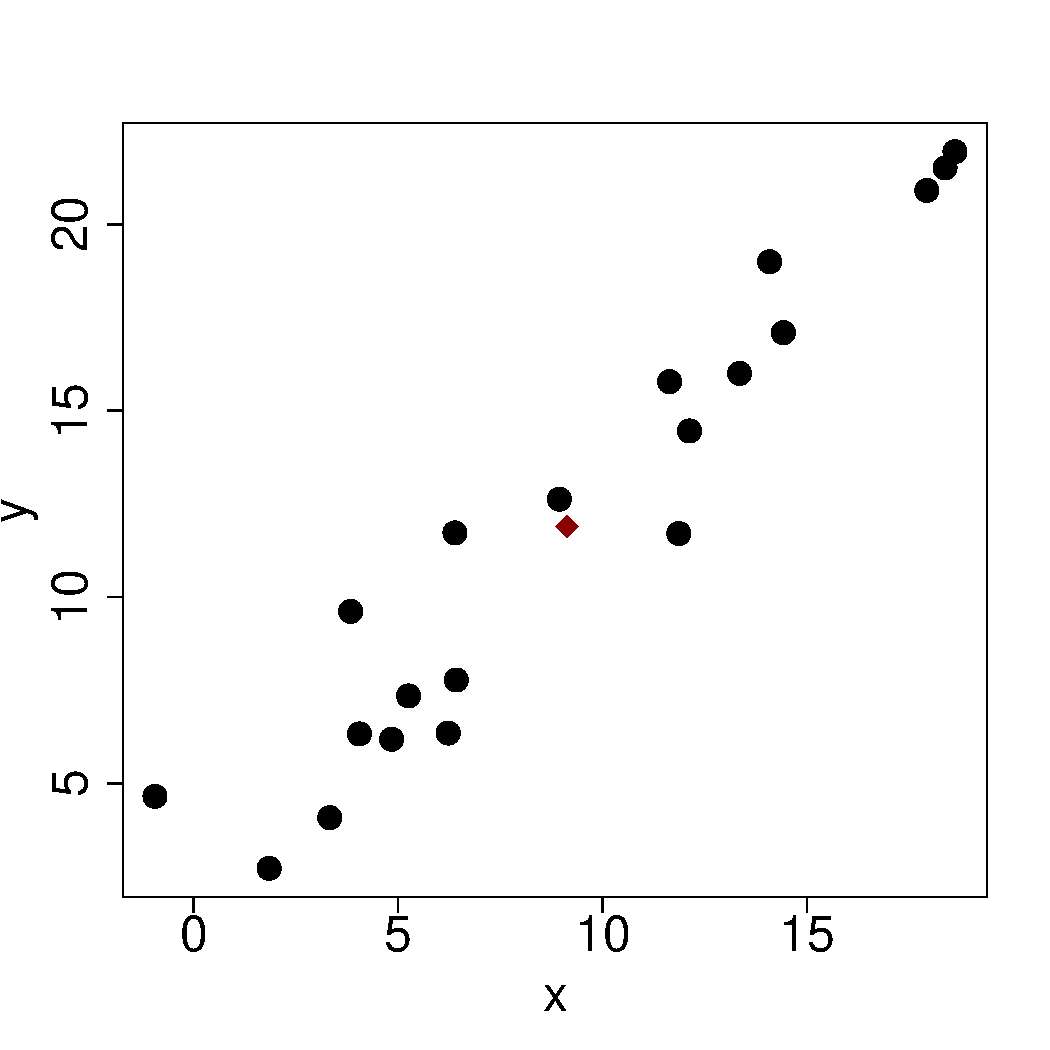
\includegraphics[height=0.7\textheight]{graphics/cov02}
  \end{center}
\end{frame}


\begin{frame}
  {Kovarianz | Illustration 2}
  Punktvarianzen | $x_3-\bar{x}=-7.81$ und $y_3-\bar{y}=-5.80$ | \alert{$-7.81\cdot-5.80=45.30$}\\
  \begin{center}
    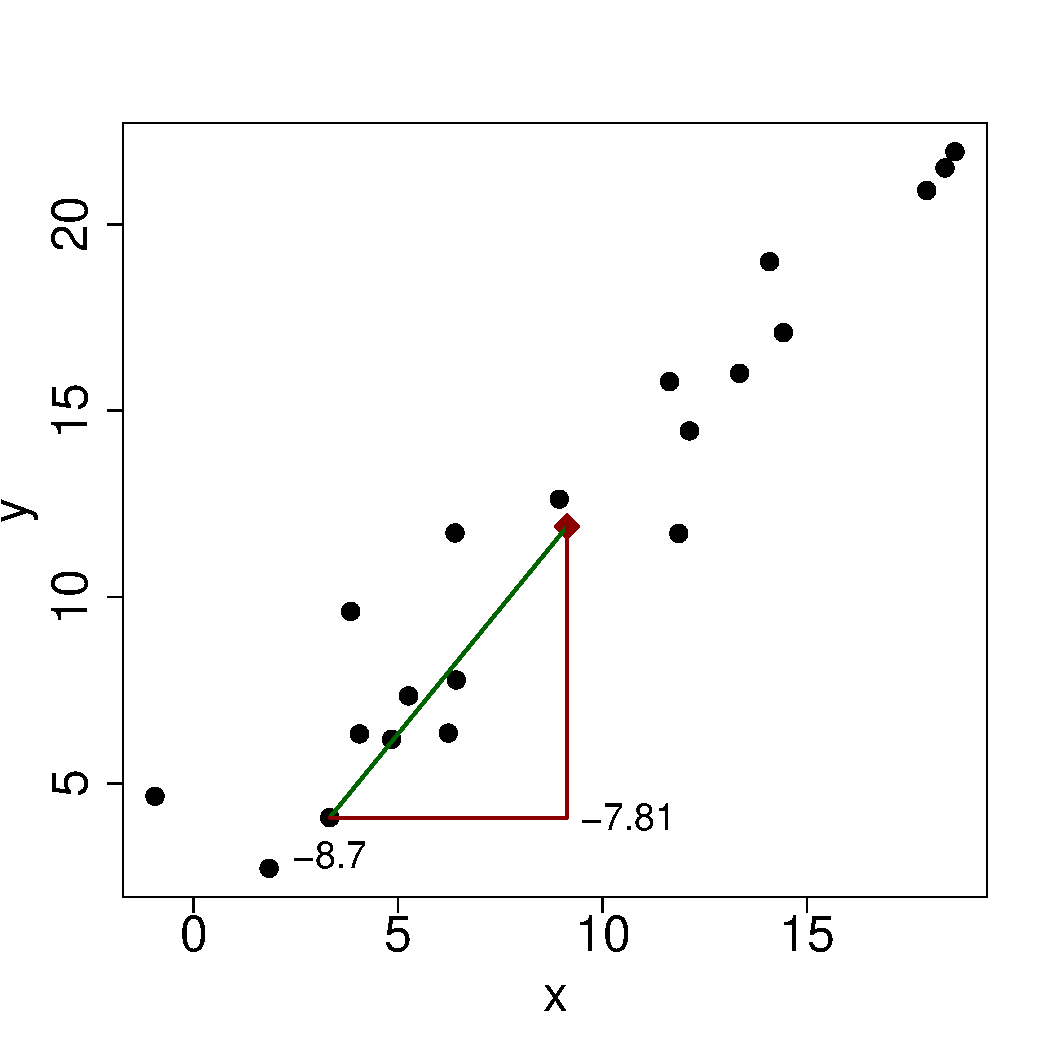
\includegraphics[height=0.7\textheight]{graphics/cov03}
  \end{center}
\end{frame}


\begin{frame}
  {Kovarianz | Illustration 3}
  Punktvarianzen | $x_{17}-\bar{x}=4.95$ und $y_{17}-\bar{y}=7.11$ | \alert{$4.95\cdot7.11=35.19$}\\
  \begin{center}
    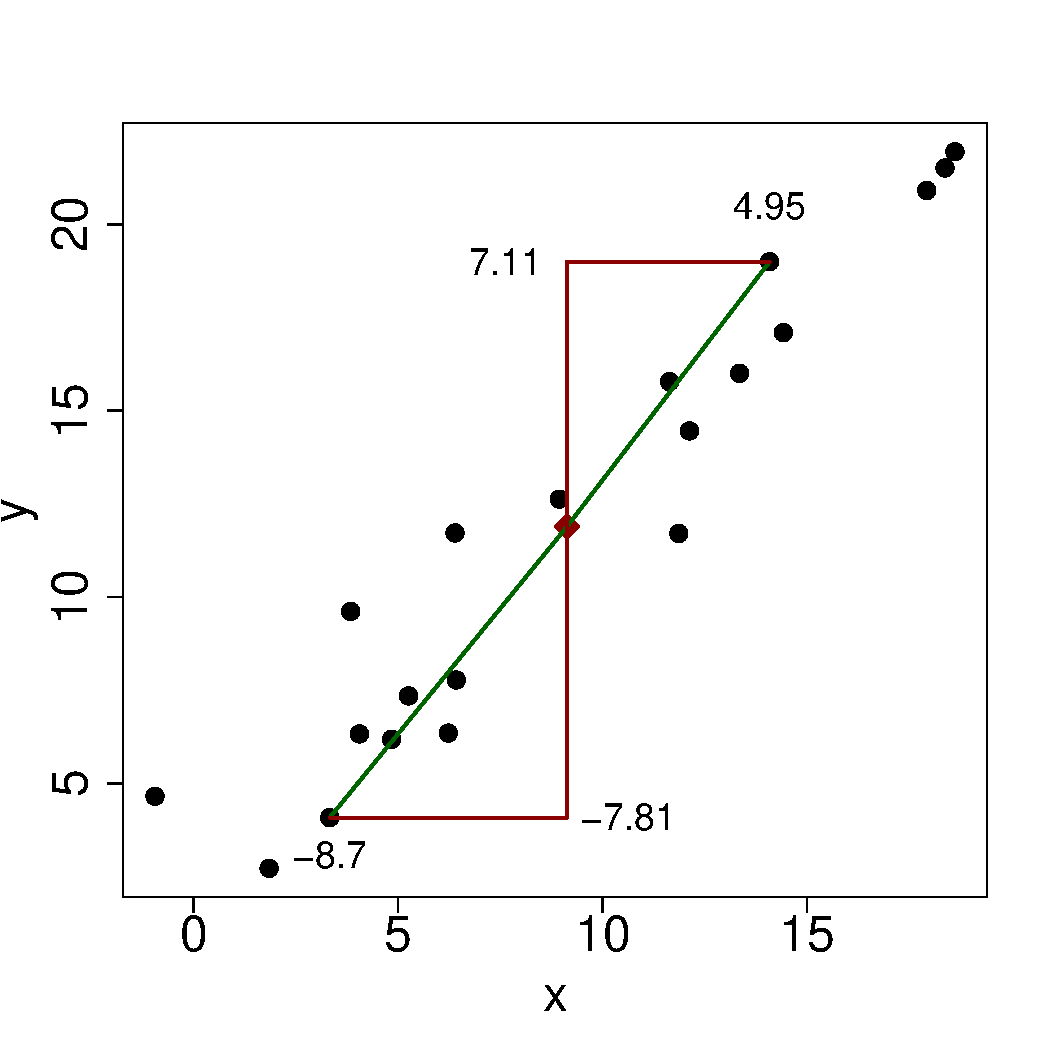
\includegraphics[height=0.7\textheight]{graphics/cov04}
  \end{center}
\end{frame}


\begin{frame}
  {Kovarianz | Illustration 4}
  Puntvarianzen für alle $\langle x_i,y_i\rangle$ \ $cov(x,y)=34.52$\\
  \begin{center}
    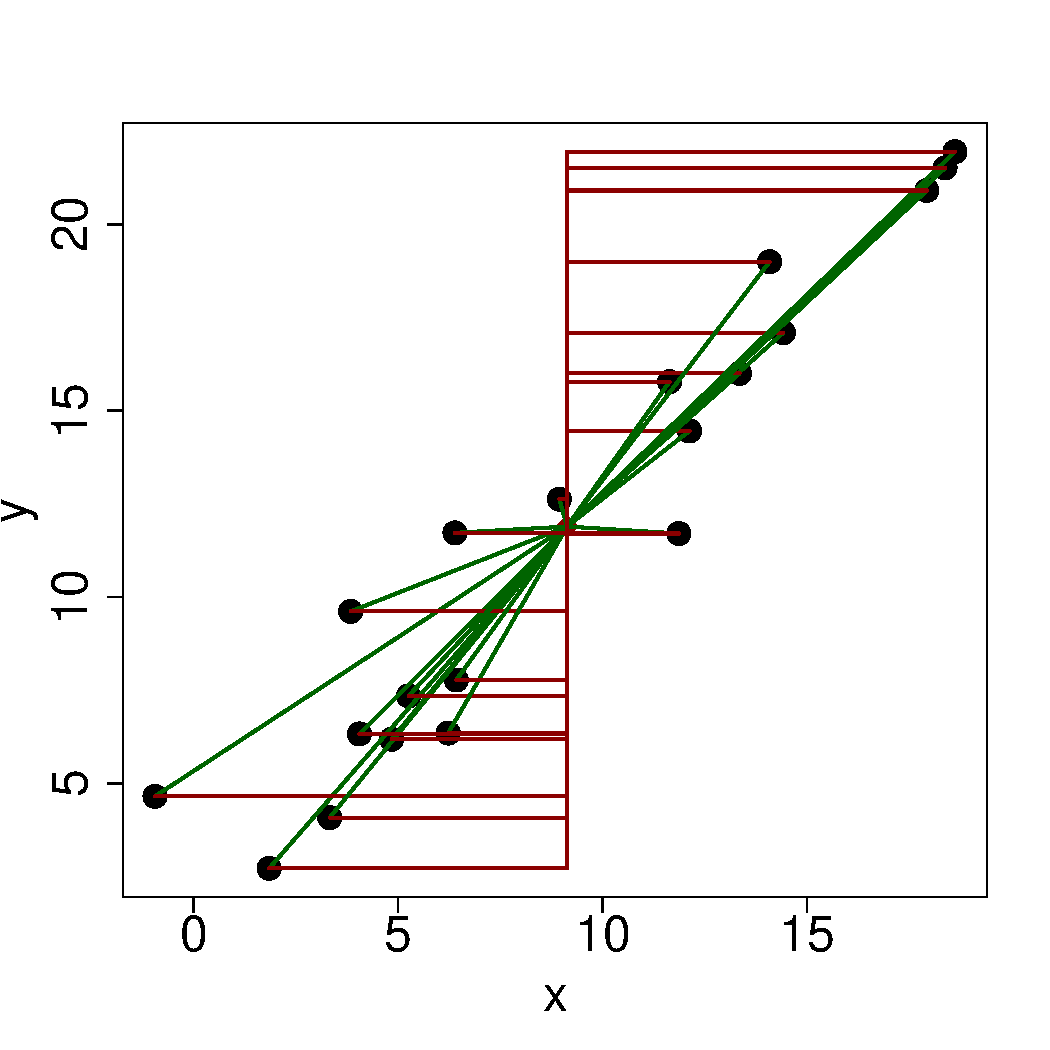
\includegraphics[height=0.7\textheight]{graphics/cov05}
  \end{center}
\end{frame}


\begin{frame}
  {Kovarianz | Illustration 5}
  Ausreißer bei ansonsten positiver Kovarianz | \alert{Negatives Produkt} der Punktvarianzen\\
  \begin{center}
    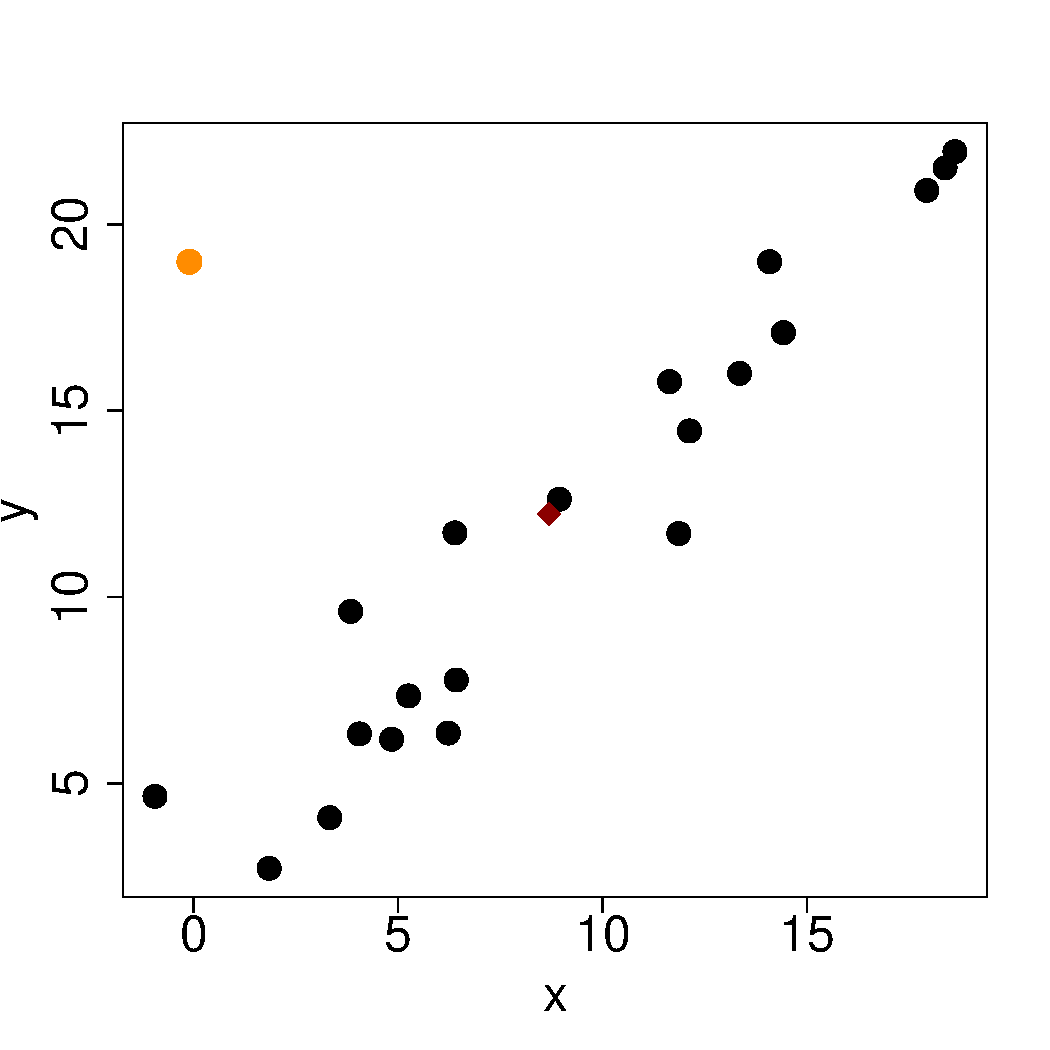
\includegraphics[height=0.7\textheight]{graphics/cov06}
  \end{center}
\end{frame}


\begin{frame}
  {Kovarianz | Illustration 6}
  Punktvarianzen | $x_{21}-\bar{x}=6.77$ und $y_{21}-\bar{y}=-8.79$ | \alert{$6.77\cdot-8.79=-59.51$}\\
  \begin{center}
    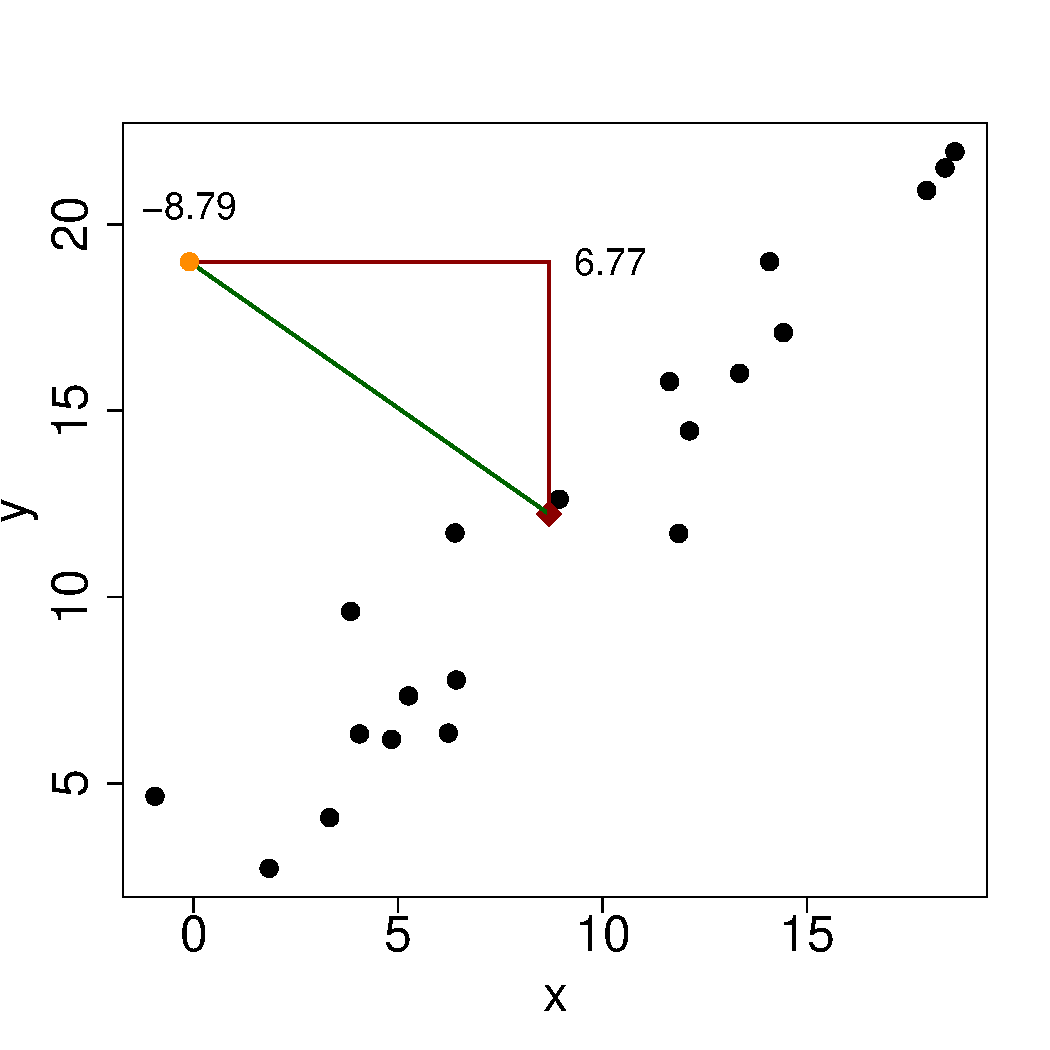
\includegraphics[height=0.7\textheight]{graphics/cov07}
  \end{center}
\end{frame}

\begin{frame}
  {Negative Kovarianz}
  Tendenziell negative Abhängigkeit | Punktvarianzen überwiegend | $cov(x,y)=-33.77$\\
  \begin{center}
    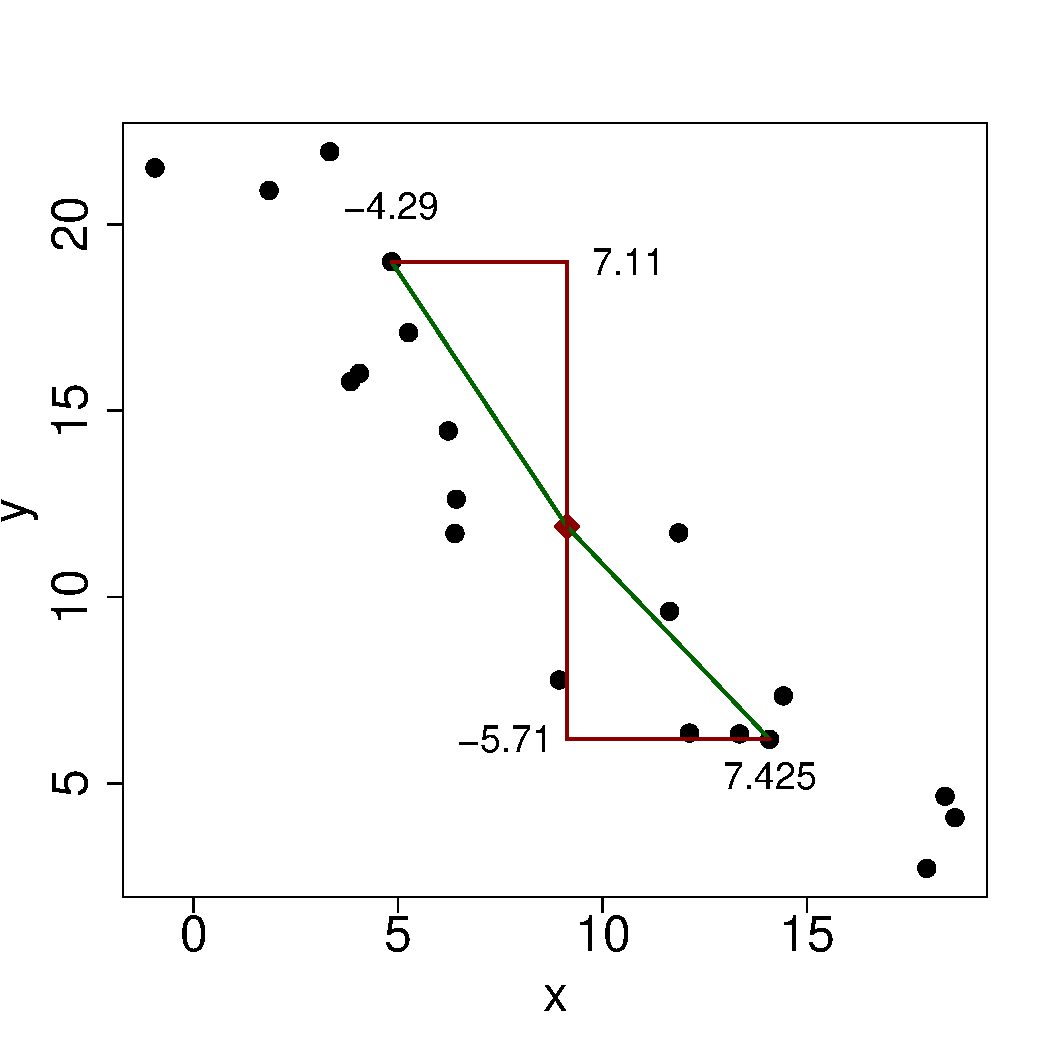
\includegraphics[height=0.7\textheight]{graphics/cov08}
  \end{center}
\end{frame}

\begin{frame}
  {Kovarianz nahe Null}
  Ohne Abhängigkeit | Kovarianz nahe 0 |$cov(x,y)=-1.74$\\
  \begin{center}
    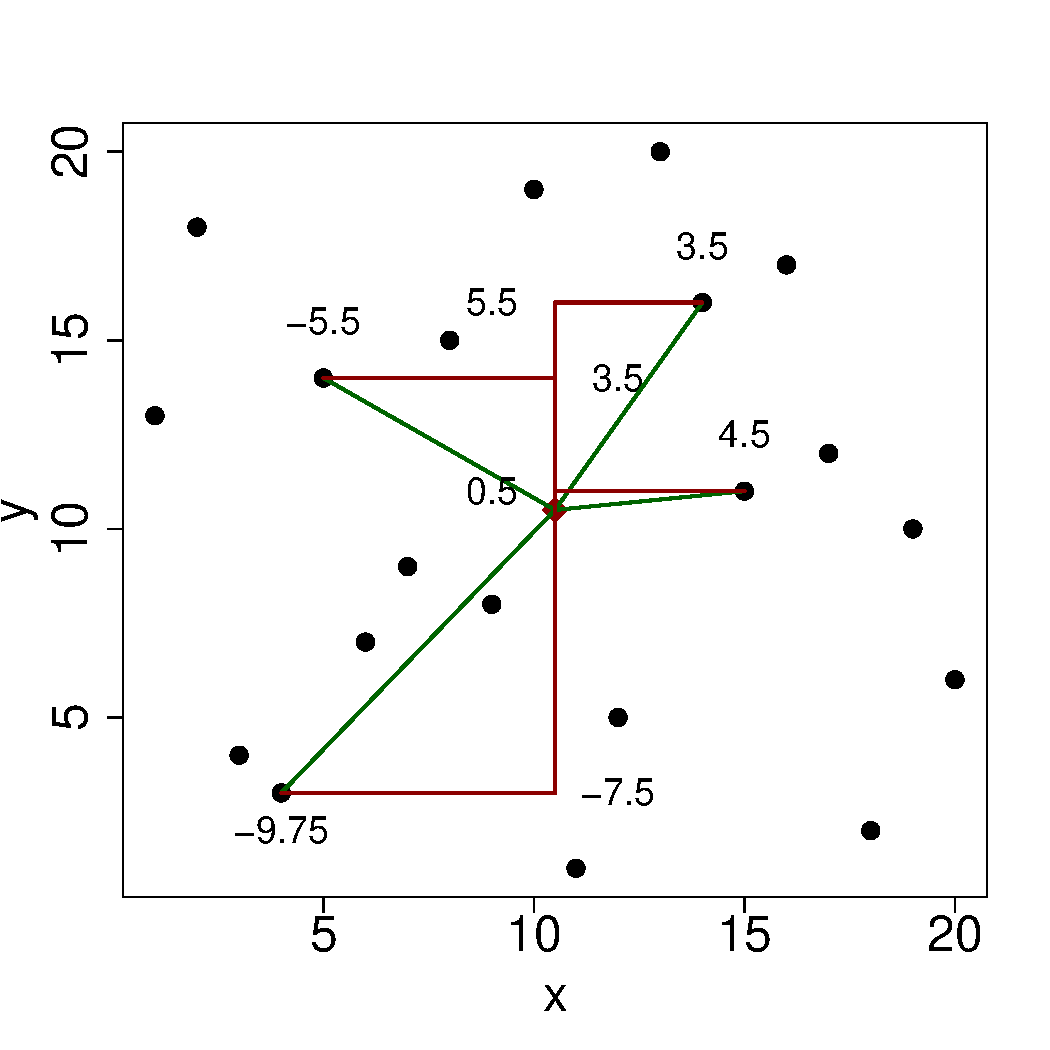
\includegraphics[height=0.7\textheight]{graphics/cov09}
  \end{center}
\end{frame}

\begin{frame}
  {Kovarianz}
  \alert{Kovarianz} | Kombination der Abweichung der Messpunkte vom jeweiligen Mittel\\
  \begin{center}
    \alert{$cov(x,y)=\frac{\sum\limits_{i=1}^{n}(x_i-\bar{x})\cdot(y_i-\bar{y})}{n-1}$}\\
    \Halbzeile
    \alert{Summe der Produkte} | Der Zählerterm | $SP(x,y)=\sum\limits_{i=1}^{n}(x_i-\bar{x})\cdot(y_i-\bar{y})$
  \end{center}
  \Halbzeile
  \begin{itemize}[<+->]
    \item \gruen{$x_i-\bar{x}>0$} und \gruen{$y_i-\bar{y}>0$} | Beitrag zur Kovarianz \gruen{positiv}
    \item \orongsch{$x_i-\bar{x}<0$} und \orongsch{$y_i-\bar{y}<0$} | Beitrag zur Kovarianz \gruen{positiv}
      \Halbzeile
    \item \gruen{$x_i-\bar{x}>0$} und \orongsch{$y_i-\bar{y}<0$} | Beitrag zur Kovarianz \orongsch{negativ}
    \item \orongsch{$x_i-\bar{x}<0$} und \gruen{$y_i-\bar{y}>0$} | Beitrag zur Kovarianz \orongsch{negativ}
  \end{itemize}
\end{frame}



\begin{frame}
  {Korrelationskoeffizient}
  \alert{Korrelationskoeffizient} | Im Gegensatz zur Kovarianz \alert{skalenunabhängig}\\
  \vspace{3\baselineskip}
  \begin{center}
    $r(x,y)=\frac{cov(x,y)}{s(x)\cdot s(y)}$\\
    \Zeile
    \grau{Pearson-Korrelation}
  \end{center}
\end{frame}




% \begin{frame}
%   {Pearson-Korrelation (Wh.)}
%   \begin{center}
%     \alert{$r(x_1,x_2)=\frac{cov(x_1,x_2)}{s(x_1)\cdot s(x_2)}$}
%   \end{center}
%   \pause
%   In Gravetter \& Wallnau, Kap.\ 16 lautet die Formel:
%   \begin{center}
%     \alert{$r=\frac{SP}{\sqrt{SQ_x\cdot SQ_y}}$}
%   \end{center}
%   Die Formeln sind äquivalent, weil (mit $x,y$ statt $x_1,x_2$):
%   \begin{center}
%     $r(x,y)=\frac{cov(x,y)}{s(x)\cdot s(y)}=\onslide<3->{\frac{\frac{\sum(x_i-\bar{x})\cdot(y_i-\bar{x})}{n-1}}{\sqrt{\frac{\sum(x_i-\bar{x})}{n-1}\cdot\frac{\sum(y_i-\bar{y})}{n-1}}}=}\onslide<4->{\frac{\frac{SP(x,y)}{n-1}}{\sqrt{\frac{\sum(x_i-\bar{x})\cdot\sum(y_i-\bar{y})}{n-1}}}=}$\\[3ex]
%     $\onslide<5->{\frac{\frac{SP(x,y)}{n-1}}{\ \ \ \frac{\sqrt{\sum(x_i-\bar{x})\cdot\sum(y_i-\bar{y})}}{n-1}\ \ \ }=}\onslide<6->{\frac{SP(x,y)}{n-1}\cdot\frac{n-1}{\sqrt{SQ(x)\cdot SQ(y)}}=}\onslide<7->{\frac{SP(x,y)}{\sqrt{SQ(x)\cdot SQ(y)}}}$
%   \end{center}
% \end{frame}

\begin{frame}
  {$r^2$ und Siginifikanztests}
  \begin{itemize}[<+->]
    \item Maß der Varianzerklärung durch $r$: \alert{$r^2$} (vgl. t-Test)
    \item \alert{Signifikanztest} möglich: Schluss auf Korrelation in der Grundgesamtheit
    \item $df_r=n-2$
    \item Unter der \Null\ (keine Korrelation) t-verteilt:\\
      \alert{$t=r\sqrt{\frac{n-2}{1-r^2}}$}
    \item \dots oder Tabellen (\zB\ G\&W, B.6)
  \end{itemize}
\end{frame}

\begin{frame}
  {Voraussetzungen}
  \begin{itemize}[<+->]
    \item \alert{Intervallskalierung}
    \item \alert{lineare} Abhängigkeit
    \item bei kleinen $n$: \alert{Normalverteilung} für $x$ und $y$
      \vspace{1cm}
    \item wenn nicht: \alert{Spearmans Rang-Korrelation}
  \end{itemize}
\end{frame}

\begin{frame}
  {Spearmans Rang-Korrelation}
  \begin{itemize}[<+->]
    \item mathematisch \alert{nicht andere als eine Pearson-Korrleation}
    \item vorher: Umrechnung der rohen x,y-Werte in \alert{Ränge}
    \item bei gleichen Werten: \alert{alle gleichen Werte bekommen Rang-Mittel}
  \end{itemize}
\end{frame}

\begin{frame}
  {Werte in Ränge umrechnen}
  Ein Beispiel zur Umwandlung in Ränge:
  \begin{center}
    \begin{tabular}[h!]{|c||c|c|c|c|c|}
      \hline
      Index: & 1 & 2 & 3 & 4 & 5 \\
      \hline
      \hline
      Messwerte x:& 4 & 7 & 3 & 1 & 3 \\
      \hline
      Messwerte y: & 9 & 12 & 11 & 2 & 8 \\
      \hline
    \end{tabular}
  \end{center}
  Statt der Messwerte arbeitet man mit den Rängen der Messwerte an den jeweiligen Indexen.
  \begin{center}
    \begin{tabular}[h!]{|c||c|c|c|c|c|}
      \hline
      Index: & 1 & 2 & 3 & 4 & 5 \\
      \hline
      \hline
      Ränge der Messwerte x:& 4 & 5 & 2.5 & 1 & 2.5 \\
      \hline
      Ränge der Messwerte y: & 3 & 5 & 4 & 1 & 2 \\
      \hline
    \end{tabular}
  \end{center}
\end{frame}

\begin{frame}
  {Abkürzung der Berechnung}
  Wenn $Rang(x_i)$ der Rang für $x_i$ in $x$ ist:\\
  \vspace{0.5cm}
  \begin{center}
    Spearmans Rang-Korrelation:\\[2ex]
    \alert{$r_{S}=1-\frac{6\sum\limits_{i=1}^n(Rang(x_i)-Rang(y_i))^2}{n(n^2-1)}$}
  \end{center}
\end{frame}

\subsection{Lineare Regression}

\begin{frame}
  {Unterschiede zwischen Korrelation und Regression}
  \begin{itemize}[<+->]
    \item Korrelation: Stärke des Zusammenhangs
    \item \alert{Regression: genaue Funktion zur Modellierung des Zusammenhangs}
      \vspace{0.5cm}
    \item Korrelation: Diagnostik\slash Test
    \item \alert{Regression: Vorhersage} (und Test)
  \end{itemize}
\end{frame}

\begin{frame}
  {Spezifikation der Funktion für die Regressionsgerade}
  \vspace{-0.5cm}
  \begin{center}
    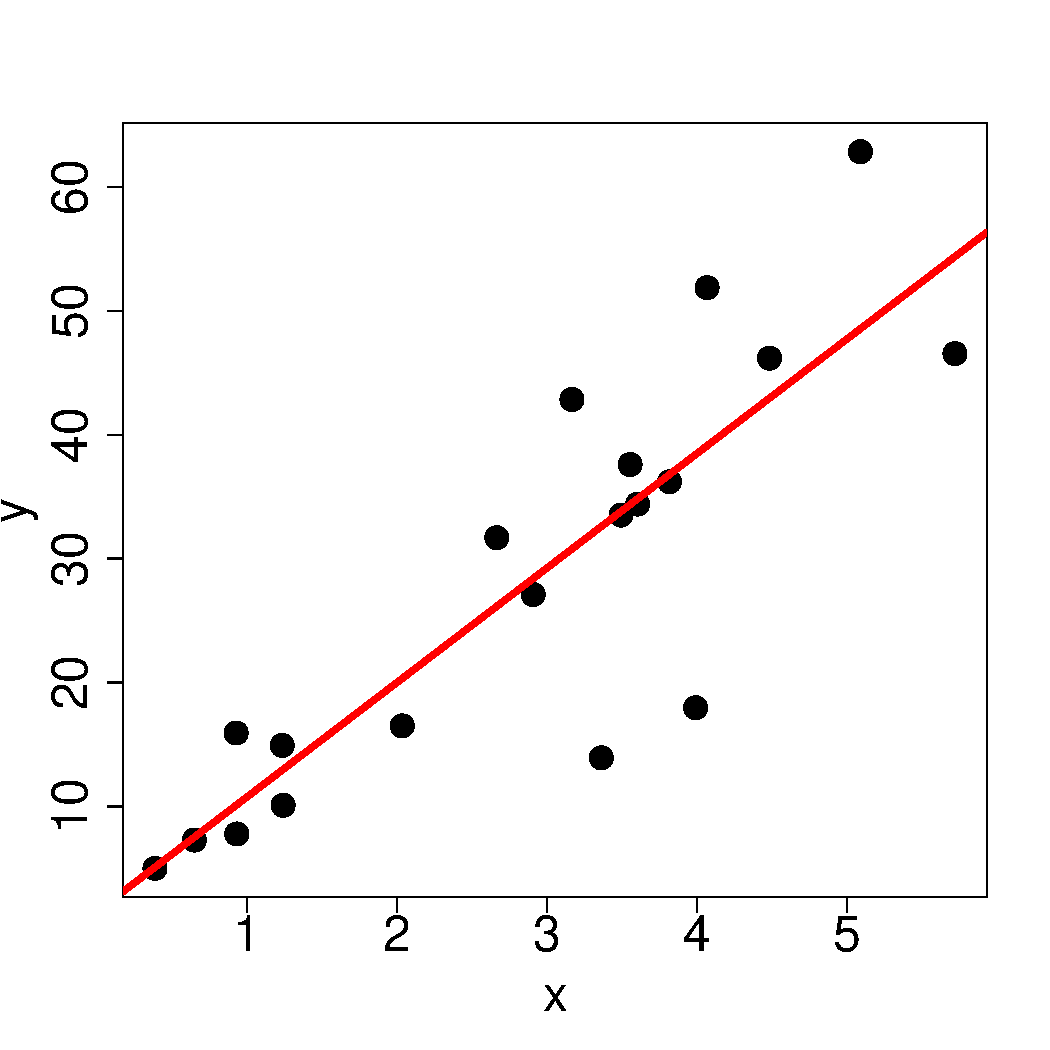
\includegraphics[width=0.3\textwidth]{graphics/regline}
  \end{center}
  \vspace{-0.5cm}
  \pause
  \begin{itemize}[<+->]
    \item Schnittpunkt mit der y-Achse (\alert{Intercept}): \alert{$a$}
    \item Steigung (\alert{Slope}): \alert{$b$} ($b$ heißt auch \alert{Koeffizient}) 
    \item \alert{Regressiongleichung (=Modell): $\hat{y}=b\cdot x+a$}
    \item Für jeden beobachteten Wert: \alert{$y_i=b\cdot x_i+a+e_i$} ($e_i$ als Fehlerterm)
  \end{itemize}
\end{frame}

\begin{frame}
  {Idee der kleinsten Quadrate}
  Die vom Modell vorhergesagten Werte (rot, auf der Regressionsgerade)\\
  sollen insgesamt einen so geringen Abstand wie möglich\\
  zu den Beobachtungen (blau) haben.
  \vspace{-0.5cm}
  \begin{center}
    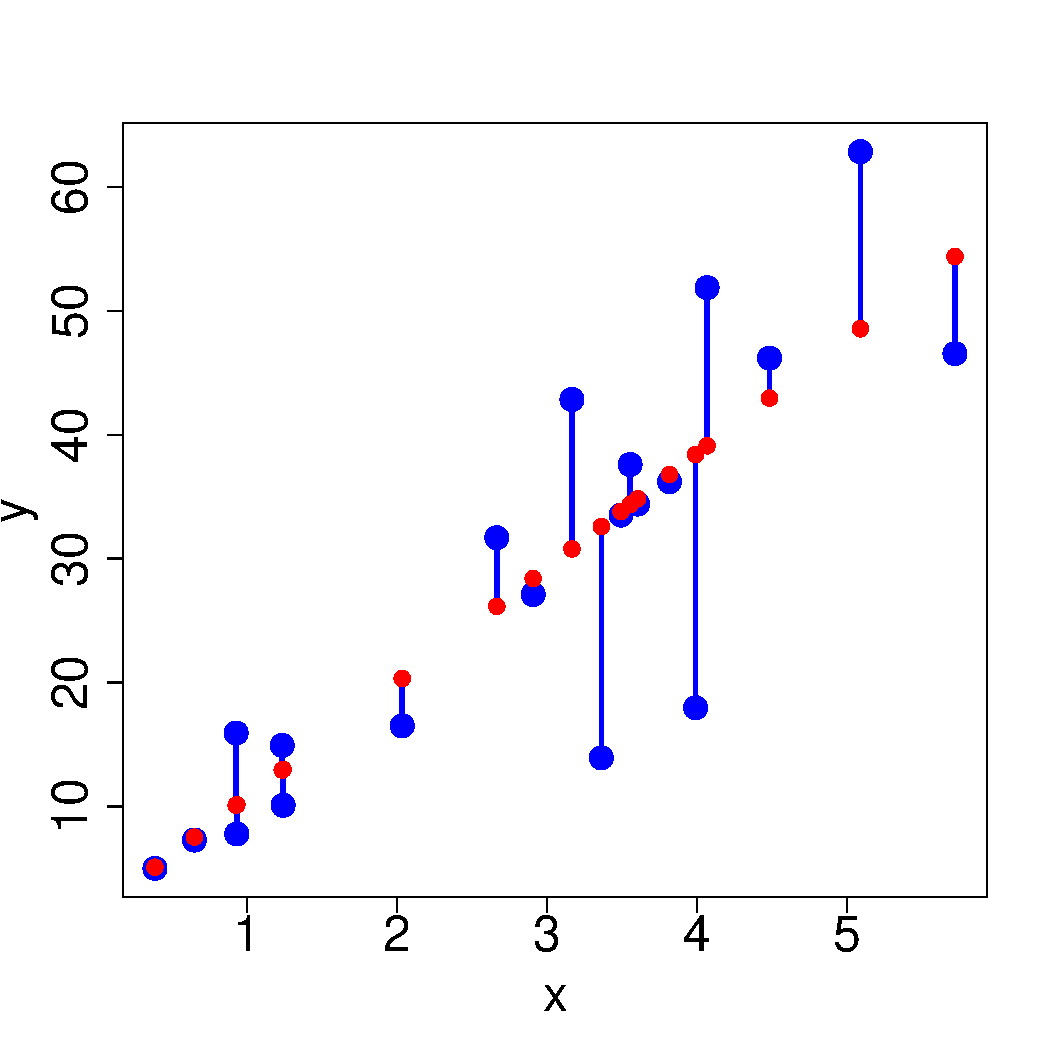
\includegraphics[width=0.3\textwidth]{graphics/lmerrors}
  \end{center}
  \pause
  Die Summe der \alert{quadrierten} negativen und positiven Differenzen (blau)\\
  soll \alert{minimiert} werden (=kleinste Quadrate): Minimierung von \alert{$E=\sum e^2$}
\end{frame}

\begin{frame}
  {Berechnung der Regressionsgleichung}
  \begin{itemize}[<+->]
    \item Slope\slash Steigung: $\alert{b=\frac{\sum(x_i-\bar{x})\cdot(y_i-\bar{y})}{\sum(x_i-\bar{x})^2}}=\frac{SP(x,y)}{SQ(x)}$
      \vspace{0.5cm}
    \item Intercept: $\alert{a=\bar{y}-b\cdot\bar{x}}$
      \vspace{0.5cm}
    \item Der Beweis, dass dies die Gerade mit den kleinsten Quadraten schätzt,
      erfordert bereits erheblichen mathematischen Aufwand, den wir uns sparen.
      \vspace{0.5cm}
    \item Determinationskoeffizient: \alert{$r^2=\frac{\sum(\hat{y}_i-\bar{y})^2}{\sum(y_i-\bar{y})^2}$}
    \end{itemize}
\end{frame}

\begin{frame}
  {Standardfehler für die Gleichung}
  \begin{itemize}[<+->]
    \item Wie stark variiert der Fehler für Stichproben einer Größe?
      \vspace{0.5cm}
    \item \alert{$SF_{residual}=\sqrt{\frac{\sum e^2}{n-2}}$}
      \vspace{0.5cm}
    \item Je kleiner $SF_{residual}$, desto besser das Modell.
    \item Beachte: $n$ wird größer (größere Stichprobe): $SF_{residual}$ wird kleiner.
    \item Und: Fehler $e$ werden kleiner: $SF_{residual}$ wird kleiner.
  \end{itemize}
\end{frame}

\begin{frame}
  {F-Test für Model}
  \begin{itemize}[<+->]
    \item Wie bei ANOVA: \alert{$F=\frac{erklaerte\ Varianz}{zufaellige\ Varianz}=\frac{s^2_{regression}}{s^2_{residual}}$}
      \vspace{0.5cm}
    \item zufällige Varianz: \alert{$s^2_{residual}=\frac{(1-r^2)\cdot SQ(y)}{1}$}
    \item erklärte Varianz: \alert{$s^2_{regression}=\frac{r^2\cdot SQ(y)}{n-2}$}
      \vspace{0.5cm}
    \item Freiheitsgrade sind immer $df_1=1$ und $df_2=n-1$.
    \item Beachte: $r^2$ ist in $[0..1]$ und teilt die Varianz von $y$ auf.
  \end{itemize}
\end{frame}

\begin{frame}
  {Standardfehler und t-Test für Koeffizienten}
  \begin{itemize}[<+->]
    \item Für $b$ und $a$ kann je ein Standardfehler angegeben werden. 
      \vspace{0.5cm}
    \item \alert{$SF(b)=\frac{\sqrt{\frac{\sum e^2}{n-1}}}{\sqrt{SQ(x)}}$}
      \vspace{0.5cm}
    \item Unter der \Null: $b=0$ ist dann t-verteilt:\\
      \alert{$t=\frac{b}{SF(b)}$}
  \end{itemize}
\end{frame}

\subsection{Multiple Regression}

\begin{frame}
  {Mehrere unabhängige}
  \begin{itemize}[<+->]
    \item Design bei einfachem LM:
      \begin{itemize}[<+->]
	\item \alert{eine intervallskalierte Abhängige}
	\item \alert{eine Unabhängige}
      \end{itemize}
      \vspace{0.5cm}
    \item wie bei mehrfaktorieller ANOVA:
      \begin{itemize}[<+->]
	\item oft interessiert \alert{mehrfaktorielle Abhängigkeit}
      \end{itemize}
  \end{itemize}
\end{frame}

\begin{frame}
  {Multivariate Modellgleichung}
  Mehrere Koeffizienten im \alert{allgemeinen linearen Modell}:\\
  \pause
  \vspace{0.5cm}
  \begin{center}
    \alert{$\hat{y}=b_1\cdot x_1+b_2\cdot x_2\dots b_n\cdot x_n+a$}
  \end{center}
  \vspace{0.5cm}
  \pause
  Konzeptuell bleibt die Berechnung aller Werte und Tests gleich,\\
  die Mathematik wird ungleich komplizierter.\\
  \vspace{0.5cm}
  \pause
  Man schreibt \alert{$R^2$} statt $r^2$.
\end{frame}

\begin{frame}
  {Normalitätsannahme}
  \begin{center}
    \alert{Die Residuen $E$ müssen normalverteilt sein.}\\
    (als Diagnostik für: \alert{Die Messwerte müssen normalverteilt sein.})
  \end{center}
  \begin{itemize}[<+->]
    \item Missverständnis: Test aller Residuen auf Normalität
    \item denn: \alert{Für jedes $x_i$ müssen die $e$ normalverteilt sein.}
    \item erfordert mehrere Messungen pro $x_i$ oder Intervallbildung 
    \item größere Stichproben, kleinere Probleme
    \item visuelle Diagnose: Q-Q-Plots (hier nicht behandelt)
  \end{itemize}
\end{frame}

\begin{frame}
  {Unabhängigkeit}
  \begin{center}
    \alert{Jedes $y_i$ darf nur von $x_i$ abhängen,\\
        niemals zusätzlich von $x_j$ mit $i\neq j$.}
  \end{center}
  \begin{itemize}[<+->]
    \item mathematisch: nicht-lineare Abhängigkeit
    \item konzeptuell: Zeitserien
    \item konzeptuell: Sequenzen in Texten
    \item Lösung: andere Modellspezifikation
  \end{itemize}
\end{frame}

\begin{frame}
  {Homoskedastizität}
  \begin{center}
    \alert{Die Residuen müssen homoskedastisch verteilt sein.}
  \end{center}
  \begin{itemize}[<+->]
    \item Bedeutung: Die Varianz der $e$ muss über alle $x$ homogen sein.
    \item vgl.\ die Forderung der "`Varianzhomogenität"' bei t-Test und ANOVA
  \end{itemize}
\end{frame}

\begin{frame}
  {Darstellung heteroskedastischer Residuen}
  Hier wird die Varianz der Residuen mit steigendem x immer größer.\\
  Ein lineares Modell versagt hier wegen verletzter Verteilungsannahmen.
  \begin{center}
    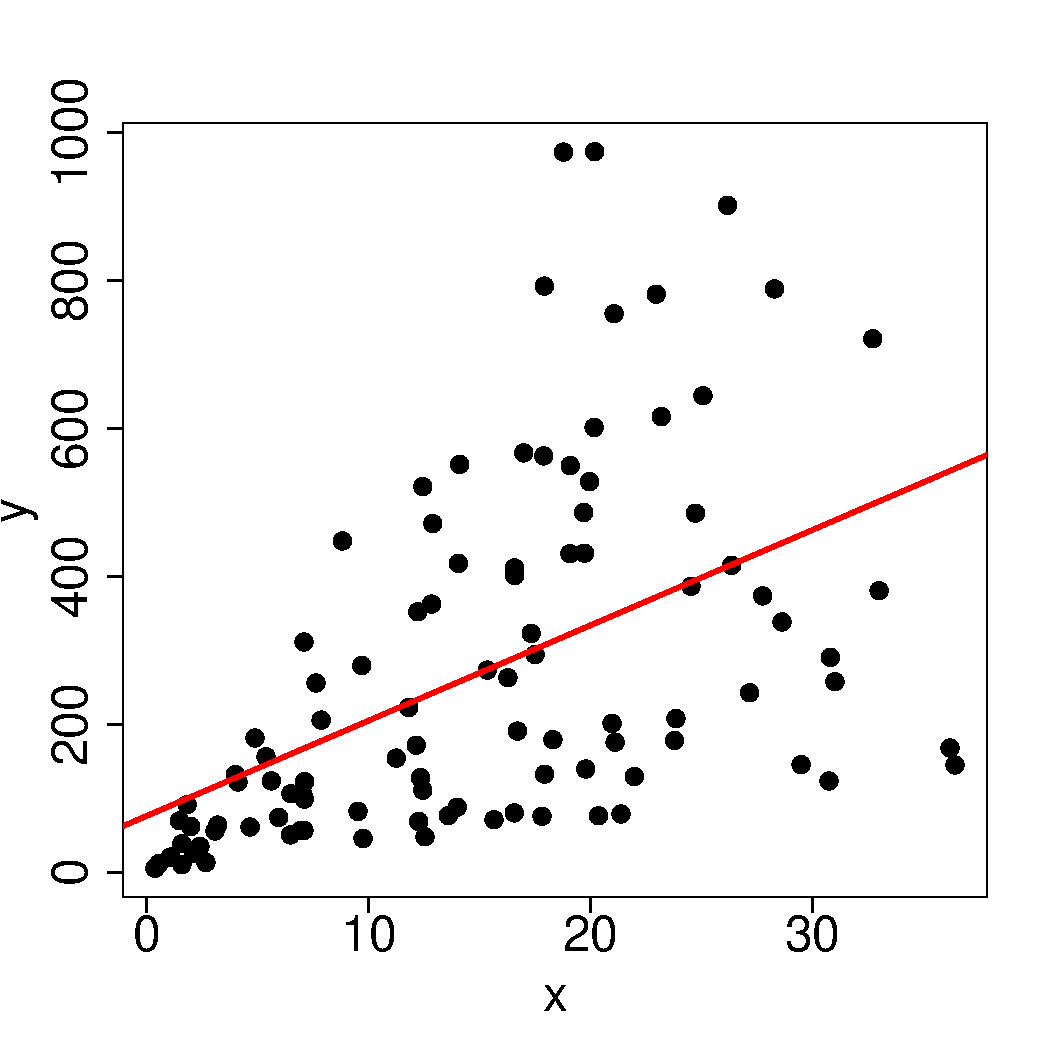
\includegraphics[width=0.4\textwidth]{graphics/hetresid}
  \end{center}
\end{frame}

\begin{frame}
  {Lösung von LM-Krisen}
  \begin{itemize}[<+->]
    \item mehr Daten ziehen, Daten transformieren
      \vspace{0.5cm}
    \item \alert{generalisierte lineare Modelle (GLM)}\\
      legen andere Verteilungsannahmen zugrunde
      \vspace{0.5cm}
    \item (generalisiert) additive Modelle (GAM)\\
      schätzen Smoothingfunktionen für Koeffizienten
  \end{itemize}
\end{frame}

\subsection{ANOVA und LMs}

\begin{frame}
  {ANOVA als Modell mit kategorialen Regressoren}
  $n$ Gruppen der ANOVA können als $n$ dichotome Variablen dargestellt werden:\\
  \vspace{0.5cm}
  \begin{center}
    \begin{tabular}[h!]{|c|c|c|c|c|}
      \cline{3-5}
      \multicolumn{2}{c|}{} & \multicolumn{3}{c|}{\textbf{ANOVA-Gruppen}} \\
      \cline{3-5}
      \multicolumn{2}{c|}{} & $A_1$ & $A_2$ & $A_3$ \\
      \hline
      \multirow{3}{*}{\begin{sideways}\textbf{Regressor}\end{sideways}} & \rule{0em}{2em} $x_1=$ & $\mathbf{1}$ & $0$ & $0$ \\
      \cline{2-5}
      & \rule{0em}{2em} $x_2=$ & $0$ & $\mathbf{1}$ & $0$ \\
      \cline{2-5}
      & \rule{0em}{2em} $x_3=$ & $0$ & $0$ & $\mathbf{1}$ \\
      \hline
    \end{tabular}
  \end{center}
\end{frame}

\begin{frame}
  {Lineares Modell mit solchen "`Dummy-Variablen"'}
  Normale Modellspezifikation:

  \begin{center}
    $\hat{y}=b_1x_1 + b_2x_2 + \cdots + b_nx_n + a$
  \end{center}
  \vspace{0.5cm}
  \pause
  \begin{center}
    Da jeweils nur eins der $x_i=1$ und alle anderen immer $0$ werden,\\
    wird einfach der Wert des entsprechenden $\beta_i$ (plus $a$) vorhergesagt.
  \end{center}
\end{frame}

%\begin{frame}
%  {Kleinste Quadrate bei Gruppen-Design}
%  Die kleinsten Quadrate erhält man in einem Design mit nominalen Abhängigen,\\
%  wenn man jeweils das Gruppen-Mittel vorhersagt.\\[03ex]
%  Wir setzen diese als Koeffizienten ein und setzen zunächst $a=0$.
%  \vspace{0.5cm}
%  \pause
%  \begin{center}
%    $\hat{y}=\bar{y_1}x_1 + \bar{y_2}x_2 + \cdots + \bar{y_n}x_n$
%  \end{center}
%  \vspace{0.5cm}
%  \pause
%  Zusätzlich kann man als Intercept das Gesamtmittel $\bar{Y}$ einsetzen\\
%  und die Koeffizienten als Abweichung vom Gesamtmittel definieren.
%  \begin{center}
%    $\hat{y}=(\bar{y_1}-\bar{Y})x_1 + (\bar{y_2}-\bar{Y})x_2 + \cdots + (\bar{y_n}-\bar{Y})x_n + \bar{Y}$
%  \end{center}
%\end{frame}
%
%\begin{frame}
%  {Beispiel}
%  Wenn $x_2=1$ (und folglich $x_1=0$ und $x_3=0$):
%  \begin{center}
%    \begin{equation}
%      \begin{split}
%	\hat{y} & = (\bar{y_1}-\bar{Y})0 + (\bar{y_2}-\bar{Y})1 + \cdots + (\bar{y_n}-\bar{Y})0 + \bar{Y}\\
%	 &= 0 + (\bar{y_2}-\bar{Y}) + \cdots + 0 + \bar{Y} \\
%	 &= \bar{y_2} - \bar{Y} + \bar{Y} \\
%	 &= \bar{y_2}
%      \end{split}
%    \end{equation}
%  \end{center}
%  \pause
%  Als Vorhersagewert kommt also einfach das $y$-Mittel der Gruppe\\
%  zum eingegebenen $x$ heraus.
%\end{frame}
%
%\begin{frame}
%  {F-Signifikanztest mit Modell-Residuen}
%  Für ein voll spezifiziertes Modell
%  \begin{center}
%    $\hat{y_f}=(\bar{y_1}-\bar{Y})x_1 + (\bar{y_2}-\bar{Y})x_2 + \cdots + (\bar{y_n}-\bar{Y})x_n + \bar{Y}$
%  \end{center}
%  \pause
%  und ein reduziertes Modell (ohne Informationen über Gruppen-Mittel)
%  \begin{center}
%    $\hat{y_r}=\bar{Y}$
%  \end{center}
%  \pause
%  können nun die Summen der Residuen verglichen werden:
%  \begin{center}
%    \alert{$F=\frac{\ \ \frac{E_r-E_f}{df_r-df_f}\ \ }{\frac{E_f}{df_f}}=\frac{\text{erklärte Varianz}}{\text{zufällige Varianz}}$}\\
%    $E_f$ = Residuen des vollen Modells, $E_r$ = Residuen des reduzierten Modells
%  \end{center}
%\end{frame}

\subsection{In \texttt{R}}

\begin{frame}
  {Spearmans Rang-Korrleation in \texttt{R}}
  Die Funktion \texttt{cor()} hat ein Argument \texttt{method},\\
  das als \texttt{"{}spearman"} angegeben werden kann.\\
  \begin{center}
    \texttt{> cor(x, y, method = "{}spearman")}
  \end{center}
\end{frame}

\begin{frame}
  {Lineare Modelle in \texttt{R}}
  \begin{itemize}[<+->]
    \item Modellformeln: \alert{\texttt{y\textasciitilde}x}\\
      "`y abhängig von x"'
    \item Mehrere Unabhängige: \alert{\texttt{y\textasciitilde x1+x2}}
    \item Mehrere Unabhängige mit \alert{Interaktion}: \alert{\texttt{y\textasciitilde x1*x2}}
    \item Mehrere Unabhängige \alert{nur Interaktion}: \alert{\texttt{y\textasciitilde x1:x2}}
      \vspace{0.5cm}
    \item Lineares Modell schätzen und speichern:\\
      \alert{\texttt{> m <- lm(y\textasciitilde x)}}
    \item Ausgabe Evaluation:\\
      \alert{\texttt{> summary(m)}}
  \end{itemize}
\end{frame}

\begin{frame}
  {Ausgabe LM}
  Interpretieren Sie diese Ausgabe anhand der Folien:\\
  \begin{center}
    \scalebox{0.7}{
    \begin{boxedminipage}{1.2\textwidth}
      \ttfamily
Call:\\
lm(formula = y \~{ } x)\\

Residuals:\\
\ \ \ \ \ Min\ \ \ \ \ \ \ 1Q\ \ \ Median\ \ \ \ \ \ \ 3Q\ \ \ \ \ \ Max\ \\
-20.4298\ \ -2.4920\ \ -0.2625\ \ \ 3.8038\ \ 14.2922\ \\

Coefficients:\\
\ \ \ \ \ \ \ \ \ \ \ \ Estimate\ Std.\ Error\ t\ value\ Pr(>|t|)\ \ \ \ \\
(Intercept)\ \ \ \ 1.513\ \ \ \ \ \ 4.321\ \ \ 0.350\ \ \ \ \ 0.73\ \ \ \ \\
x\ \ \ \ \ \ \ \ \ \ \ \ \ \ 9.242\ \ \ \ \ \ 1.333\ \ \ 6.933\ 1.77e-06\ ***\\
---\\
Signif.\ codes:\ \ 0\ ‘***’\ 0.001\ ‘**’\ 0.01\ ‘*’\ 0.05\ ‘.’\ 0.1\ ‘\ ’\ 1\\

Residual\ standard\ error:\ 9.008\ on\ 18\ degrees\ of\ freedom\\
Multiple\ R-squared:\ \ 0.7275,	Adjusted\ R-squared:\ \ 0.7124\ \\
F-statistic:\ 48.06\ on\ 1\ and\ 18\ DF,\ \ p-value:\ 1.768e-06\ \\
    \end{boxedminipage}}
  \end{center}
\end{frame}

%\begin{frame}
%  {ANOVA in \texttt{R}}
%  Beispiel: zweifaktoriella ANOVA mit Faktor A und B und Interaktion.
%  \begin{itemize}[<+->]
%    \item Modell spezifizieren:\\
%      \alert{\texttt{> m <- lm(x\textasciitilde A*B)}}
%    \item ANOVA rechnen\slash speichern:\\
%      \alert{\texttt{> a <- aov(m)}}
%    \item Ausgabe:\\
%      \alert{\texttt{> summary(a)}}
%  \end{itemize}
%\end{frame}
%
%\begin{frame}
%  {Ausgabe ANOVA}
%  \begin{center}
%    \scalebox{0.7}{
%    \begin{boxedminipage}{1.2\textwidth}
%      \ttfamily
%\ \ \ \ \ \ \ \ \ \ \ \ \ Df\ Sum\ Sq\ Mean\ Sq\ F\ value\ \ \ Pr(>F)\ \ \ \\ \
%A\ \ \ \ \ \ \ \ \ \ \ \ 1\ \ \ 0.38\ \ \ \ 0.38\ \ \ 0.094\ 0.762577\ \ \ \ \\
%B\ \ \ \ \ \ \ \ \ \ \ \ 2\ \ \ 6.25\ \ \ \ 3.12\ \ \ 0.784\ 0.471570\ \ \ \ \\
%A:B\ \ \ \ \ \ \ \ \ \ 2\ 105.25\ \ \ 52.62\ \ 13.202\ 0.000296\ ***\ \\
%Residuals\ \ \ 18\ \ 71.75\ \ \ \ 3.99\ \ \ \ \ \ \ \ \ \ \ \ \ \ \ \ \ \ \ \ \ \\
%---\\
%Signif.\ codes:\ \ 0\ ‘***’\ 0.001\ ‘**’\ 0.01\ ‘*’\ 0.05\ ‘.’\ 0.1\ ‘\ ’\ 1\\
%    \end{boxedminipage}}
%  \end{center}
%  Hinweis: Mit \texttt{"{}Mean Sq"} ist $s^2$ gemeint.
%\end{frame}


\section{Lineare Modelle und ANOVA}


\begin{frame}
  {Äquivalenz von ANOVA und LM}
  Binäre Kodierung der Gruppenzugehörigkeit\\
  Hier: drei Gruppen von einem Faktor (einfaktorielle ANOVA mit drei Gruppen)\\

 \begin{center}
   \begin{tabular}[h!]{|c|c|c|c|c|}
     \cline{3-5}
     \multicolumn{2}{c|}{} & \multicolumn{3}{c|}{\textbf{ANOVA-Gruppen}} \\
     \cline{3-5}
     \multicolumn{2}{c|}{} & $A_1$ & $A_2$ & $A_3$ \\
     \hline
     \multirow{3}{*}{\begin{sideways}\textbf{Regressor}\end{sideways}} & \rule{0pt}{18pt} $x_1=$ & $\mathbf{1}$ & $0$ & $0$ \\
     \cline{2-5}
     & \rule{0pt}{18pt} $x_2=$ & $0$ & $\mathbf{1}$ & $0$ \\
     \cline{2-5}
     & \rule{0pt}{18pt} $x_3=$ & $0$ & $0$ & $\mathbf{1}$ \\
     \hline
   \end{tabular}
  \Zeile
   \begin{equation}
    \hat{y}=b_1x_1 + b_2x_2 + \cdots + b_nx_n + a
  \end{equation}
 \end{center}
\end{frame}


\begin{frame}
  {Volles Modell, Kleinste Quadrate}
  Kleinste Quadrate | für jeden Koeffizienten $b_i$ jeweils Mittelwert der Gruppe $i$ ($\bar{y_i}$)\\
  Außerdem erstmal $a=0$ | dann:\\
  \Halbzeile 
  \begin{equation}
    \hat{y}=\bar{y_1}x_1 + \bar{y_2}x_2 + \cdots + \bar{y_n}x_n
  \end{equation}

  \Zeile
  Allgemeines Mittel als Intercept | $a=\bar{Y}$\\
  Koeffizienten = Abweichung Gruppenmittel vom Gesamtmittel\\
  \Halbzeile  
  \begin{equation}
    \hat{y}=(\bar{y_1}-\bar{Y})x_1 + (\bar{y_2}-\bar{Y})x_2 + \cdots + (\bar{y_n}-\bar{Y})x_n + \mathbf{\bar{Y}}
  \end{equation}
\end{frame}


\begin{frame}
  {Beispiel für einen Datenpunkt aus Gruppe 2}
  Entsprechend in ANOVA $A_2$ | Unabhängige im LM: $x_1=0$, $x_2=1$ und $x_3=0$\\
  Schätzung für den $y$-Wert:\\
  \Halbzeile  
  \begin{equation}
    \begin{split}
      \hat{y} & = (\bar{y_1}-\bar{Y})0 + \mathbf{(\bar{y_2}-\bar{Y})1} + \cdots + (\bar{y_n}-\bar{Y})0 + \mathbf{\bar{Y}}\\
       &= 0 + (\bar{y_2}-\bar{Y}) + \cdots + 0 + \bar{Y} \\
       &= \bar{y_2} - \bar{Y} + \bar{Y} \\
       &= \bar{y_2}
    \end{split}
  \end{equation}
  
  \Zeile
  Jeder $\hat{y}$-Wert | Mittel der beobachteten $y$-Werte der Gruppe, zu der er gehört\\
  \grau{\footnotesize Das ergibt für ausschließlich nominale Unabhängige in der Tat den Schätzer mit den kleinsten Quadraten (s.\ Maxwell \& Delaney, Kap.\ 3).}
\end{frame}

\begin{frame}
  {Test über Modell}
  Kernfrag | \alert{Bringen Abweichungen der Gruppenmittel eine Verbesserung der Vorhersage\\
  gegenüber dem Gesamt-Mittel?}\\
  \Halbzeile
  Methode | Vergleich der \alert{Residuen $E_f$ für volles Modell} (mit Gruppenmitteln)\\
  vs.\ \alert{Residuen $E_r$ für reduziertes Modell} (ohne Gruppenmittel)\\

  \Zeile
  Gleichung~\ref{eq:fullmod} für volles und Gleichung~\ref{eq:redmod} für reduziertes Modell\\
  
  \begin{equation}
      \mathbf{\hat{y_f}}=(\bar{y_1}-\bar{Y})x_1 + (\bar{y_2}-\bar{Y})x_2 + \cdots + (\bar{y_n}-\bar{Y})x_n + \bar{Y}
      \label{eq:fullmod}
  \end{equation}
  
  \begin{equation}
    \mathbf{\hat{y_r}}=\bar{Y}
      \label{eq:redmod}
  \end{equation}
  
\end{frame}

\begin{frame}
  {Vergleich von Varianzen = ANOVA | F-Verteilung}
  \begin{equation}
    F=\frac{\ \ \frac{E_r-E_f}{df_r-df_f}\ \ }{\frac{E_f}{df_f}}=\frac{\text{erklärte Varianz}}{\text{zufällige\ Varianz}}
  \end{equation}

  \Zeile
  \begin{enumerate}
    \item Residuen = Maß für die Varianz
    \item Residuen des vollen Modells = Maß für die Varianz,\\
      die trotz der Erklärungskraft des vollen Modells bleibt (= unerklärte Varianz)
    \item Residuen des reduzierten Modells = Maß für die Gesamtvarianz\\
      (Abweichungen vom Gesamt-Mittel)
    \item Zähler | trotz der Erklärung verbleibende Varianz $-$ vollen Varianz\\
      abgezogen (=  erklärte Varianz)
    \item Quotient insgesamt | Zählervarianz in Bezug zur Gesamtvarianz\\
      (klassischer F-Quotient, s.\ ANOVA)
  \end{enumerate}
\end{frame}

% Dieser Vergleich erfolgt über den folgenden F-Quotienten, mit dem konzeptuell und mathematisch die Konvergenz zur klassischen ANOVA hergestellt wird:
% 
% 
% Alternativ kann man eins der Gruppenmittel zum Referenzmittel (= Intercept) machen.
% Dann evaluiert man die anderen relativ zu diesem.
% Konzeptuell ist das dasselbe.
% 
% In \texttt{R} kann man eine ANOVA folgendermaßen Rechnen und damit eine klassische ANOVA-Ausgabe produzieren (mit \texttt{Mean Sq} meint \texttt{R} einfach die Varianz $s^2$):
% 
% \begin{center}
%   \textbf{\texttt{summary(aov(lm(y\textasciitilde A)))}}
% \end{center}
% 
% \texttt{y} ist dabei ein Vektor, der die beobachteten Werte enthält, und \texttt{A} ein Faktor, der passend dazu die Faktor-Ausprägungen entsprechend der Gruppen paart.
% Als Mini-Beispiel:
% 
% \begin{center}
%   \begin{tabular}[h!]{|c|c|c|}
%     \cline{1-1}\cline{3-3}
%     \textbf{\texttt{y}} && \textbf{\texttt{A}} \\
%     \cline{1-1}\cline{3-3}
%     \multicolumn{1}{c}{} & \multicolumn{1}{c}{} & \multicolumn{1}{c}{}\\
%     \cline{1-1}\cline{3-3}
%     0 && 1 \\
%     1 && 1 \\
%     3 && 1 \\
%     1 && 1 \\
%     \cline{1-1}\cline{3-3}
%     4 && 2 \\
%     3 && 2 \\
%     6 && 2 \\
%     3 && 2 \\
%     \cline{1-1}\cline{3-3}
%   \end{tabular}
% \end{center}





\ifdefined\TITLE
  \section{Nächste Woche | Überblick}

  \begin{frame}
    {Einzelthemen}
    \begin{enumerate}
      \item Inferenz
      \item Deskriptive Statistik
      \item Nichtparametrische Verfahren
      \item z-Test und t-Test
      \item ANOVA
      \item Freiheitsgrade und Effektstärken
      \item Power und Severity
      \item Lineare Modelle
      \item \alert{Generalisierte Lineare Modelle}
      \item Gemischte Modelle
    \end{enumerate}
  \end{frame}
\fi
